\begin{frame}
\frametitle{The Majorana landscape} 
 \begin{center}
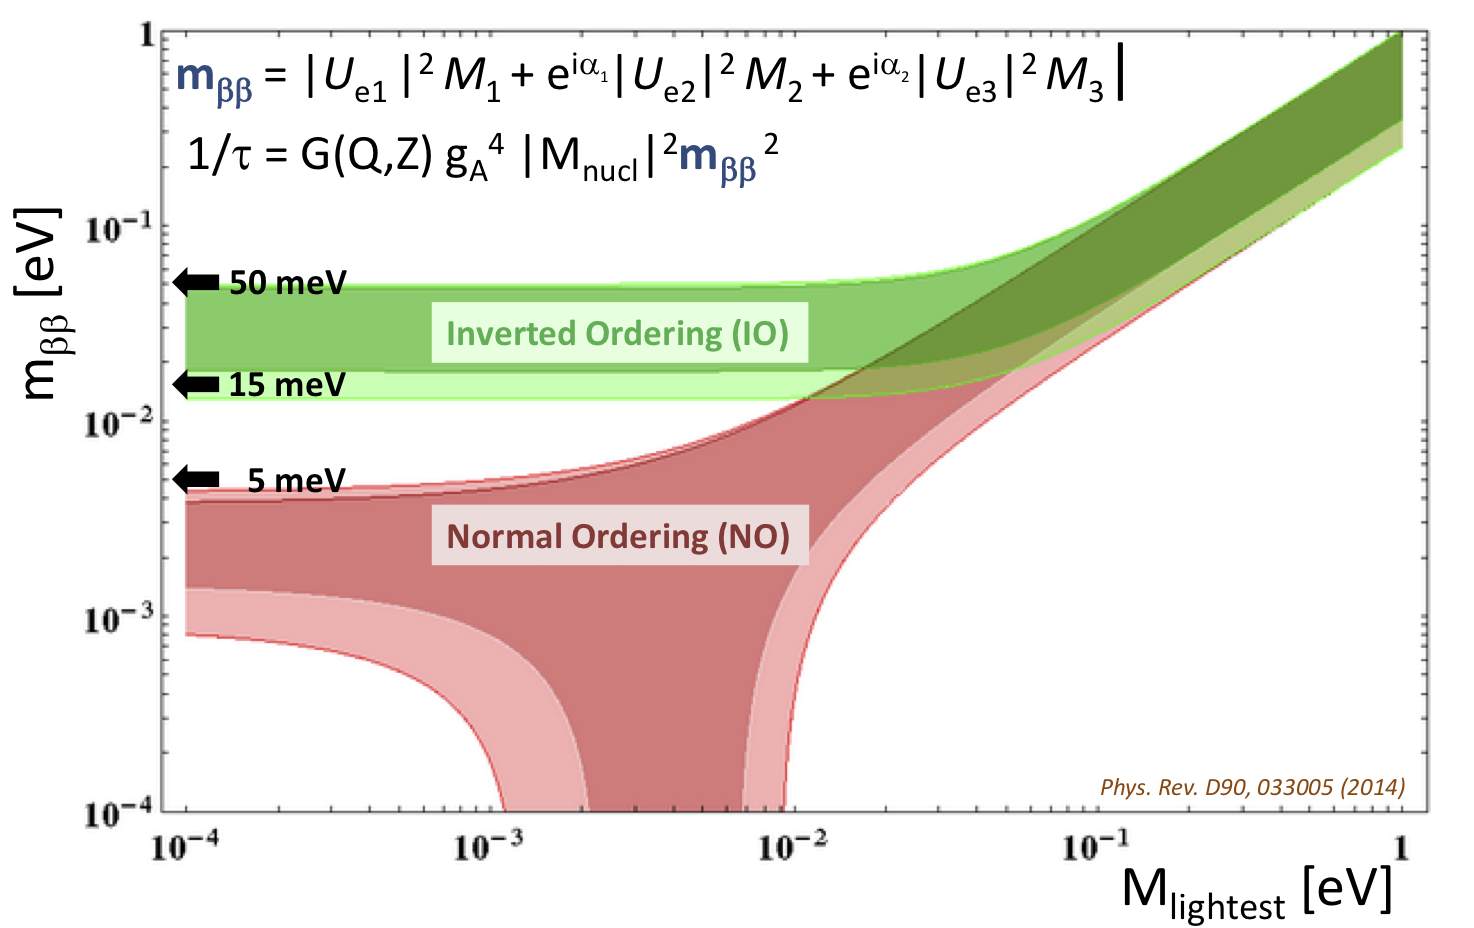
\includegraphics[width=0.75\textwidth]{moriond/landscape.png}
\end{center}
\begin{itemize}
\item {\bf Majorana's  landscape} obtained when plotting \mbb\ vs the lightest neutrino mass.
\item {\bf Majorana's curse:} Sensitivity to $\mbb \propto to \sqrt{1/\tau}$.
\end{itemize}
 \begin{flushright}
{\bf A. Giuliani, Neutrino 2018}
\end{flushright}

\end{frame}

\begin{frame}
\frametitle{Connecting \mbb\ with $\tau$} 
 \begin{center}
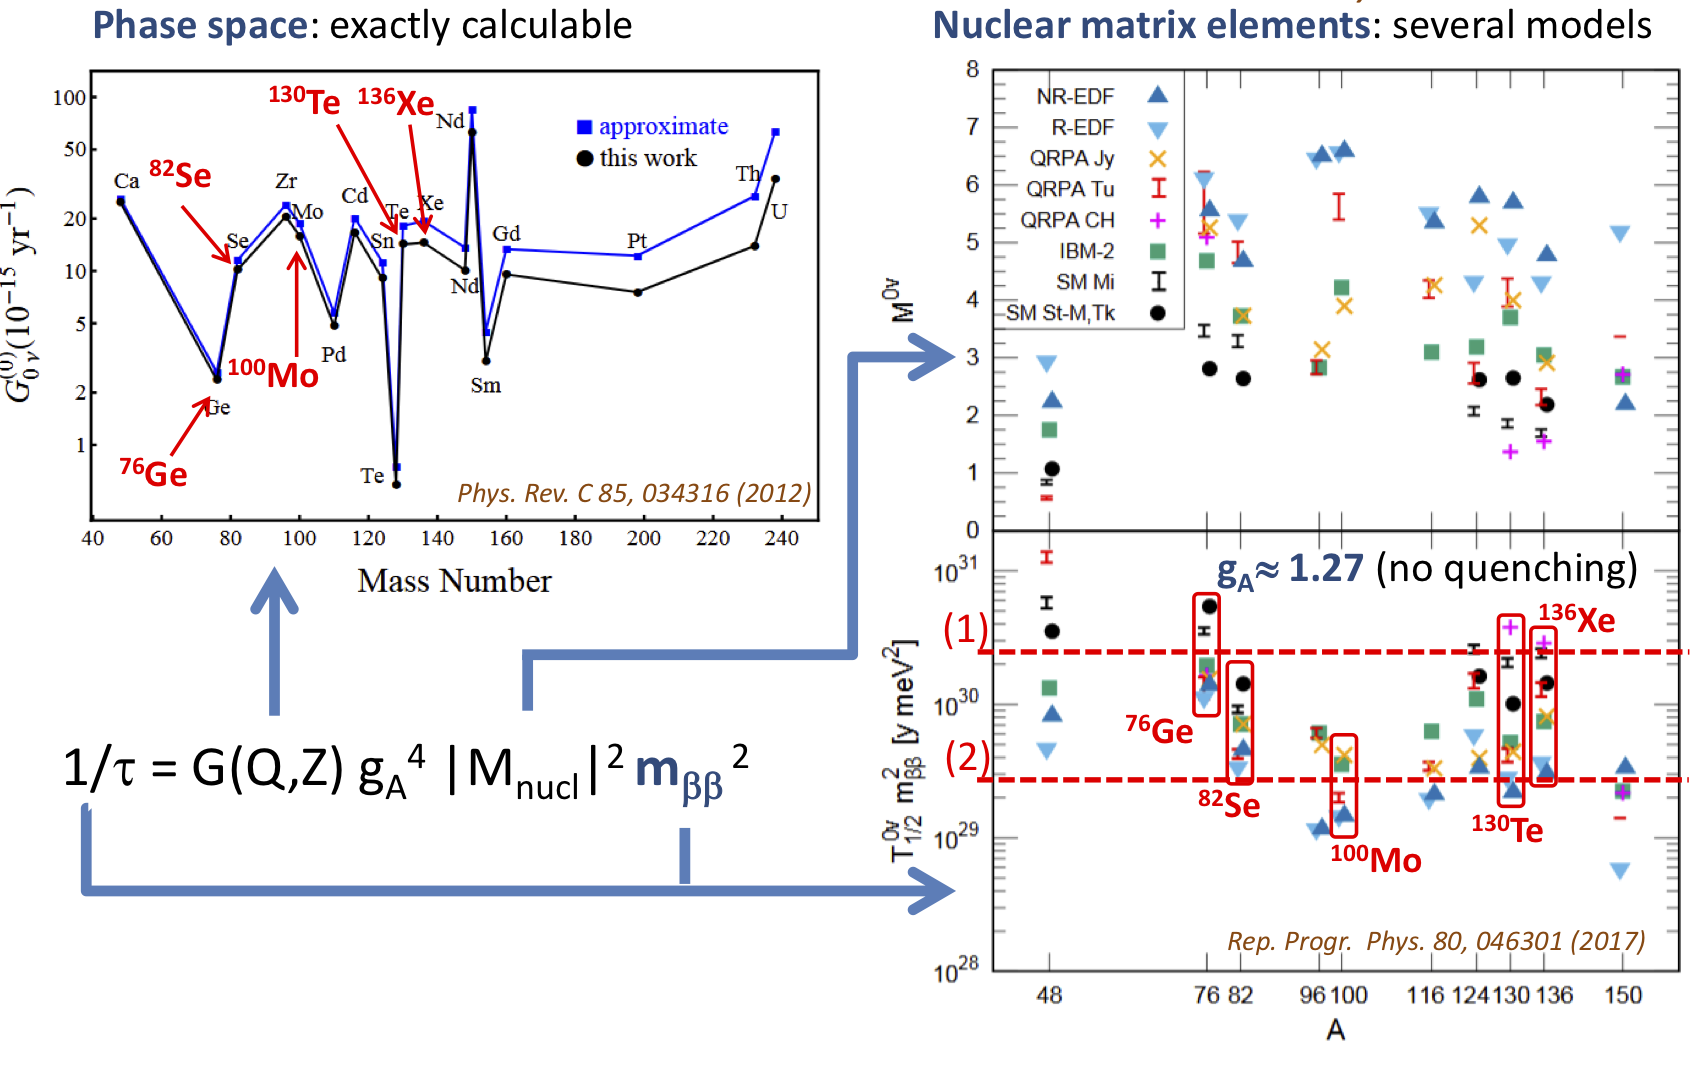
\includegraphics[width=0.75\textwidth]{moriond/nme.png}
\end{center}
\begin{itemize}
\item {\bf case (1):} ``optimistic scenario".
\item {\bf case (2):} ``pessimistic scenario".
\end{itemize}
 \begin{flushright}
{\bf A. Giuliani, Neutrino 2018}
\end{flushright}
\end{frame}

\begin{frame}
\frametitle{Setting the scale} 
 \begin{center}
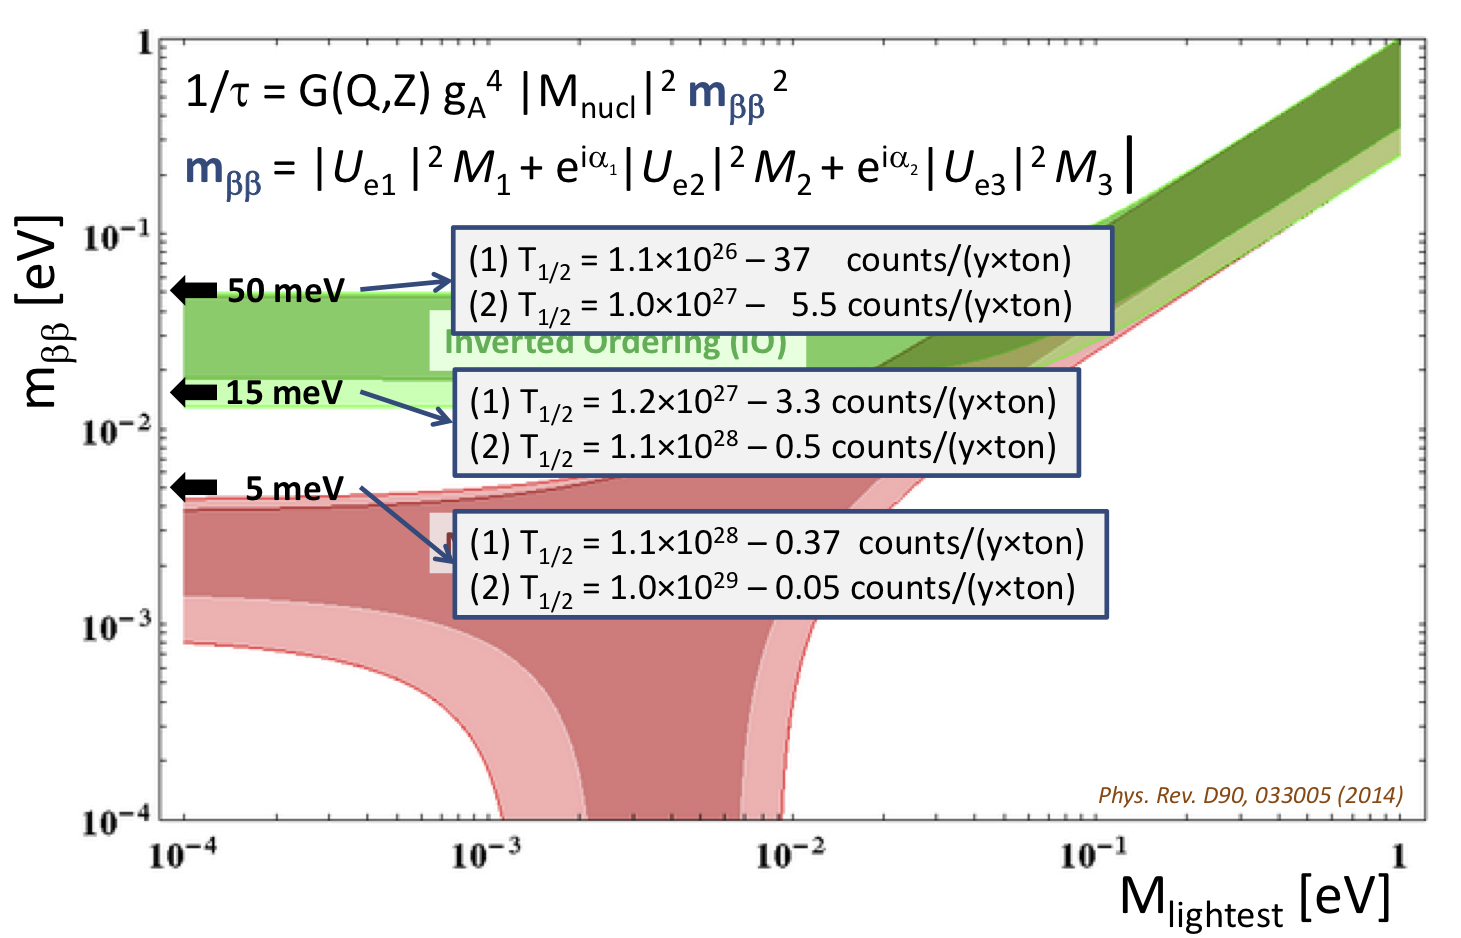
\includegraphics[width=0.75\textwidth]{moriond/setting_the_scale.png}
\end{center}
\begin{itemize}
\item {\bf case (1):}  $\Tonu \sim 10^{27} {\rm yr} \rightarrow \mbb \sim {\rm 15 meV}$, 
$\Tonu \sim 10^{28} {\rm yr} \rightarrow \mbb \sim {\rm 5 meV}$.
\item {\bf case (2):} $\Tonu \sim 10^{28} {\rm yr} \rightarrow \mbb \sim {\rm 15 meV}$, 
$\Tonu \sim 10^{29} {\rm yr} \rightarrow \mbb \sim {\rm 5 meV}$.
\end{itemize}
 \begin{flushright}
{\bf A. Giuliani, Neutrino 2018}
\end{flushright}

\end{frame}

\begin{frame}
\frametitle{Majorana's challenge}

\begin{figure}[tbh!]
  \begin{center}
      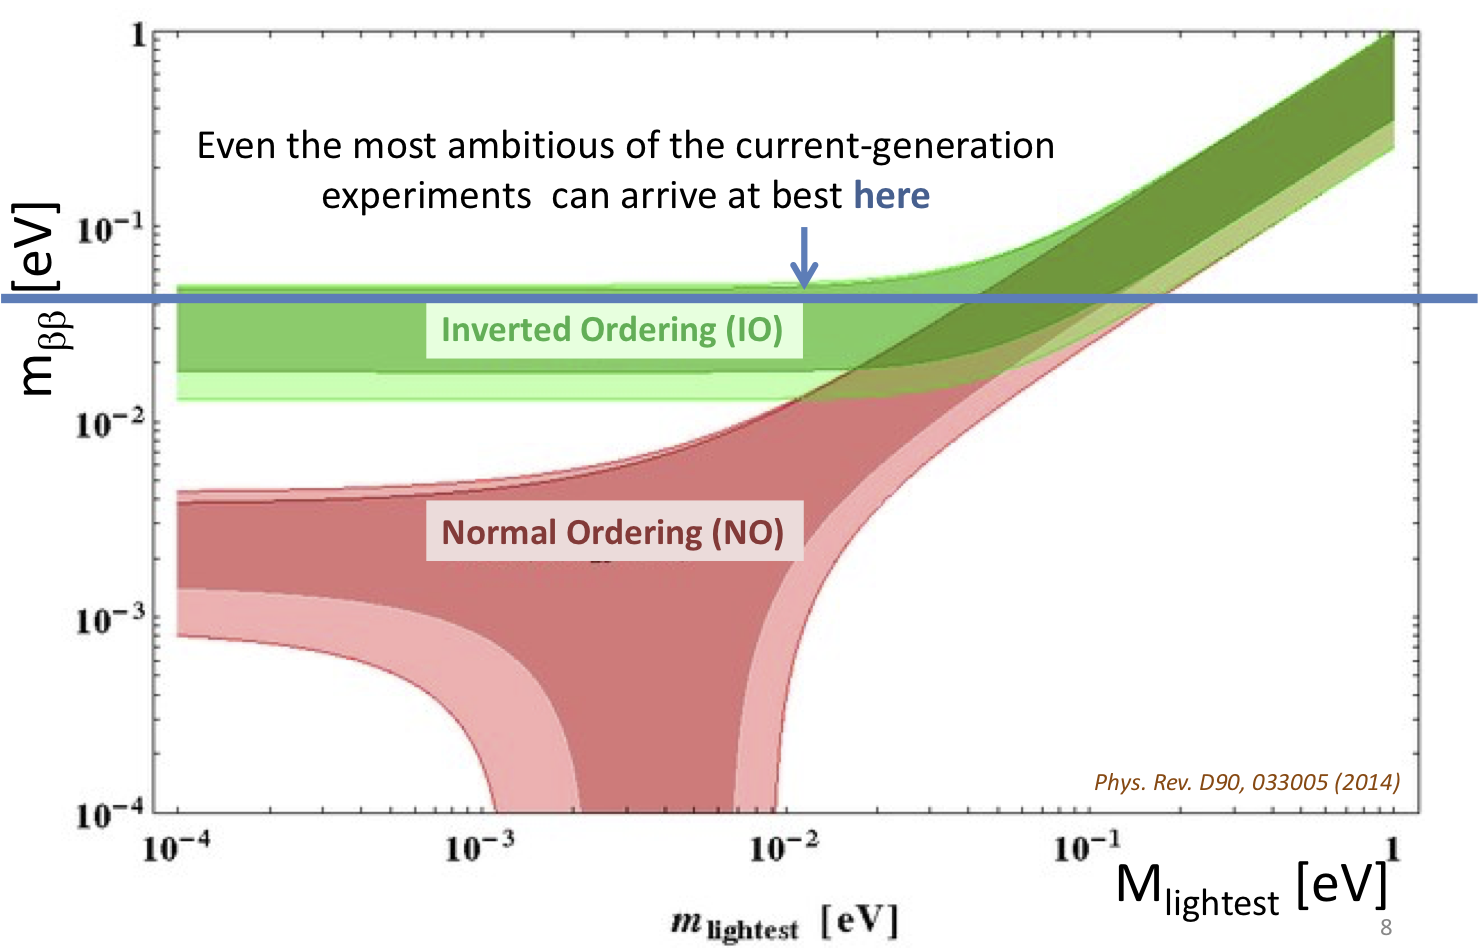
\includegraphics[width=0.45\textwidth]{moriond/current_experiments.png}
       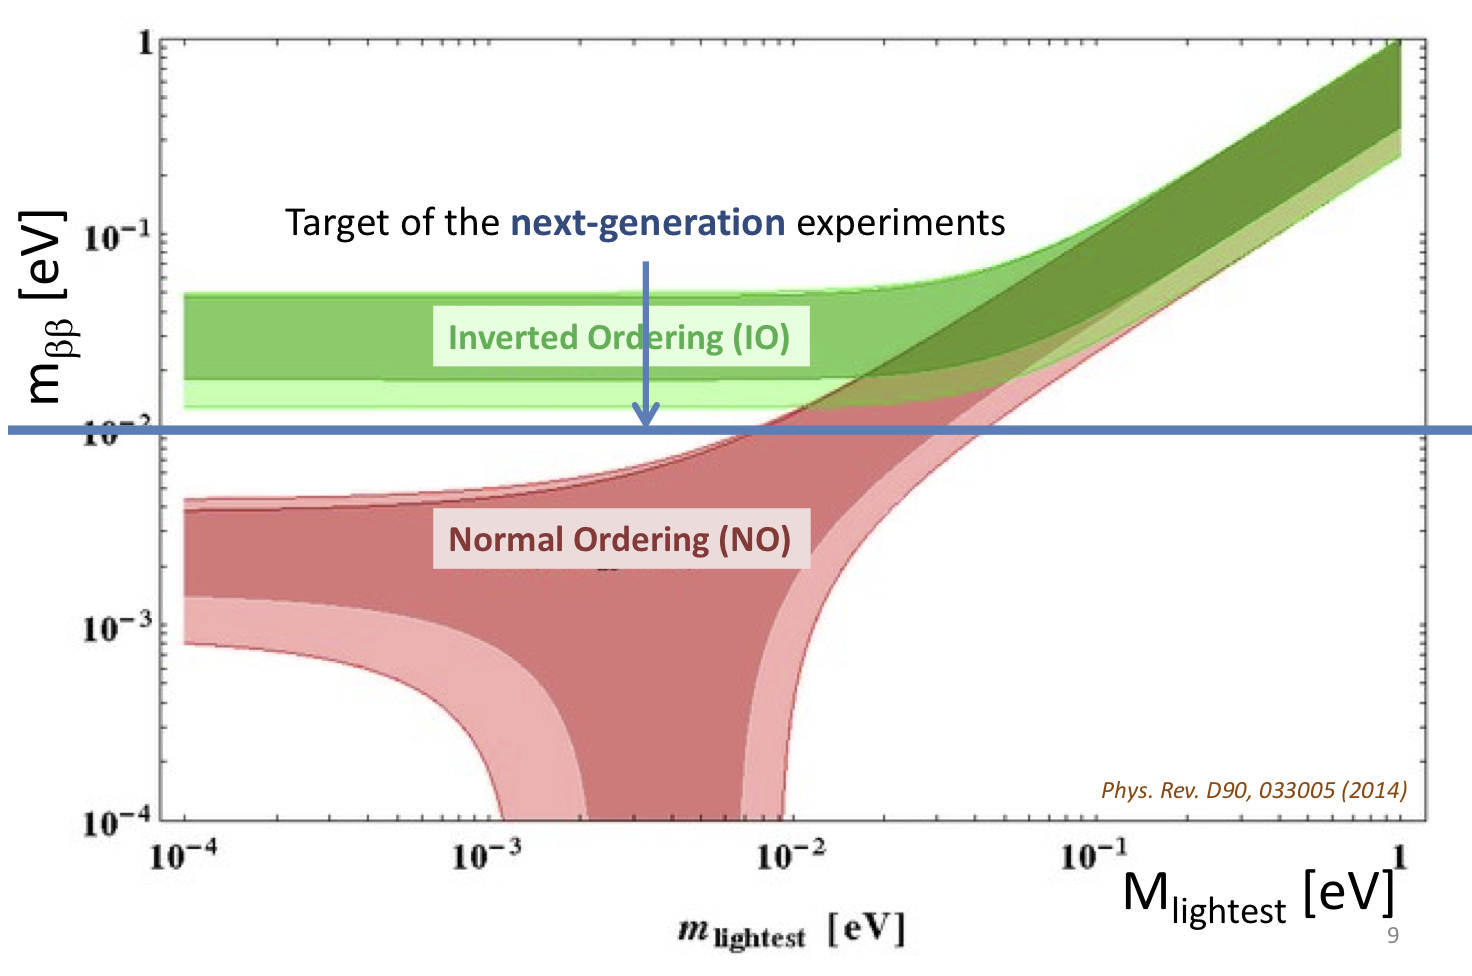
\includegraphics[width=0.45\textwidth]{moriond/nextgen_experiments.png}
      
  \end{center}
\end{figure}
\begin{itemize}
\item {\bf today:} $\Tonu \sim 10^{26} {\rm yr}$.
\item {\bf case (1):} if $\Tonu \sim 10^{27} {\rm yr}$, observe 3 signal events.
\item {\bf case (2):} if $\Tonu \sim 10^{28} {\rm yr}$, observe 0.5 signal events.
\end{itemize}
\end{frame}

\begin{frame}
\frametitle{Next generation experiments must be ``background free''}

\begin{columns}
 
\column{0.5\textwidth}
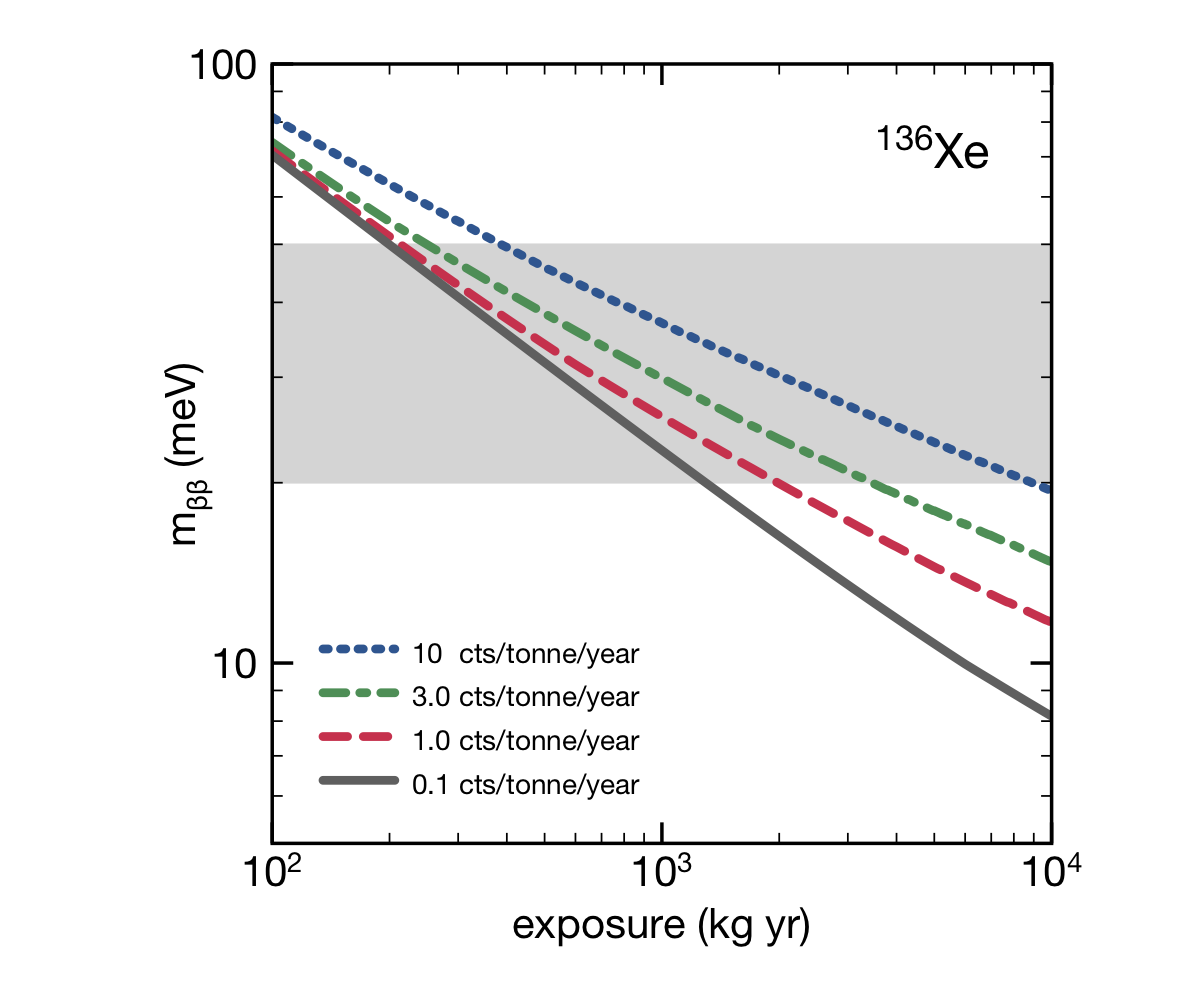
\includegraphics[scale=0.35]{moriond/xenon_bkg.png}
 
\column{0.5\textwidth}
\begin{itemize}
\item Plot shows the sensitivity of a 100\% efficient Xenon experiment assuming scenario (1).
\item With a background $\sim$ 10 \ckky\ an exposure of 10 ton years  (30 ton years for an efficiency of 30 \%) is needed to cover the IH.
\item With a background count of  $\sim$ 1 \ckky\, ``only'' 2 ton years are required (6 ton years for an efficiency of 30\%).
\item To reach 5 meV in 10 ton years requires a background free (0.1 \ckky) experiment. 
\end{itemize}
\end{columns}
\end{frame}

 





